%\title{LaTeX Portrait Poster Template}
%%%%%%%%%%%%%%%%%%%%%%%%%%%%%%%%%%%%%%%%%
% a0poster Portrait Poster
% LaTeX Template
% Version 1.0 (22/06/13)
%
% The a0poster class was created by:
% Gerlinde Kettl and Matthias Weiser (tex@kettl.de)
% 
% This template has been downloaded from:
% http://www.LaTeXTemplates.com
%
% License:
% CC BY-NC-SA 3.0 (http://creativecommons.org/licenses/by-nc-sa/3.0/)
%
%%%%%%%%%%%%%%%%%%%%%%%%%%%%%%%%%%%%%%%%%

%----------------------------------------------------------------------------------------
%	PACKAGES AND OTHER DOCUMENT CONFIGURATIONS
%----------------------------------------------------------------------------------------

\documentclass[a0,portrait]{a0poster}

\usepackage{lineno}
\usepackage{array}
\usepackage{lscape}
\usepackage{graphicx}
\usepackage{subcaption}
\usepackage{float}
\usepackage{multicol} % This is so we can have multiple columns of text side-by-side
\usepackage{amsmath}
\columnsep=100pt % This is the amount of white space between the columns in the poster
\columnseprule=3pt % This is the thickness of the black line between the columns in the poster

\usepackage[svgnames]{xcolor} % Specify colors by their 'svgnames', for a full list of all colors available see here: http://www.latextemplates.com/svgnames-colors

\usepackage{times} % Use the times font
%\usepackage{palatino} % Uncomment to use the Palatino font

\usepackage{graphicx} % Required for including images
\graphicspath{{figures/}} % Location of the graphics files
\usepackage{booktabs} % Top and bottom rules for table
\usepackage[font=small,labelfont=bf]{caption} % Required for specifying captions to tables and figures
\usepackage{amsfonts, amsmath, amsthm, amssymb} % For math fonts, symbols and environments
\usepackage{wrapfig} % Allows wrapping text around tables and figures

\newcommand{\bbbar}{$b\bar{b}$}
\newcommand{\afb}{$A_{FB}^b$}
\newcommand{\sm}{Standard Model}
\newcommand{\bsm}{Beyond Standard Model}
\newcommand{\mF}{\mathcal{F}^I}

\begin{document}

%----------------------------------------------------------------------------------------
%	POSTER HEADER 
%----------------------------------------------------------------------------------------


\begin{minipage}[b]{1.\linewidth}
\veryHuge \color{NavyBlue} \textbf{Studies of $e^+e^-\to b\bar{b}$ channel at the International Linear Collider} \color{Black} % Title
 % Subtitle
\end{minipage}
\begin{minipage}[b]{0.5\linewidth}
\Huge\textit{Final word on LEP \afb\ anomaly}\\[1cm]
\huge \textbf{\underline{BILOKIN S.}, P\"OSCHL R., RICHARD F.}\\[0.5cm] % Author(s)
\huge Laboratoire de l'Acceler\'ateur Lin\'eare\\[0.4cm] % University/organization
\Large \texttt{bilokin@lal.in2p3.fr}
\end{minipage}
\begin{minipage}[b]{0.5\linewidth}
	\centering
\includegraphics[height=7cm]{figures/LAL.jpg}
\includegraphics[height=7cm]{figures/UPSUD.jpg}
\includegraphics[height=7cm]{figures/logo-ild.png}\\
\end{minipage}

\vspace{1cm} % A bit of extra whitespace between the header and poster content

%----------------------------------------------------------------------------------------

\begin{multicols}{2} % This is how many columns your poster will be broken into, a portrait poster is generally split into 2 columns

%----------------------------------------------------------------------------------------
%	ABSTRACT
%----------------------------------------------------------------------------------------

\color{Navy} % Navy color for the abstract

\begin{abstract}
The heavy quark doublet plays a central role in the quest for new physics. The complementary between studies of electroweak top quark production and bottom quark production is therefore intuitively clear and pointed out in the literature. Let us remind that the tension between the LEP measurement and the Standard Model prediction of the forward-backward asymmetry \afb\ is still one of the unsolved questions in the field and may be interpreted as a first manifestation of new physics in the heavy quark sector. The process $e^+e^-\to b\bar{b}$ at the ILC offers a unique opportunity for a final word on the tension. Polarised beams allow for a large disentangling of the coupling constants or form factors that govern the $Z^0/\gamma b \bar{b}$ vertex.

This poster presents a detailed simulation study of the process $e^+e^-\to b\bar{b}$ at 250\,GeV with the ILD Detector. Besides the phenomenological implications, the studies demonstrate that with a careful analysis of the final state the charge of the b-quarks can be determined on an event-by-event basis with the ILD Detector. Such a capability is unprecedented by past and present particle physics experiments.
\end{abstract}

%----------------------------------------------------------------------------------------
%	INTRODUCTION
%----------------------------------------------------------------------------------------

\color{SaddleBrown} % SaddleBrown color for the introduction

\section*{Introduction}

So far, LEP~I has determined the b-quark couplings to the $Z^0$ boson by measuring the b partial width 
and the forward-backward asymmetry called \afb. 
These quantities provide the most precise value of $\sin^2\theta_W$ at LEP~I. It turns out that this value is at three standard deviation away from the very precise value from SLD using beam polarization~\cite{bib:AfbSMFit}. 
Redoing precisely this measurement is therefore a priority for future e+e‐ colliders. 


In this study, we intend to prove that the International Linear Collider~\cite{bib:ILC}, with polarized beams and 
high luminosity, offers a unique opportunity for precise measurements well above the resonance, where both $Z^0$ and photon exchanges are present. 
This additional complexity may turn up to be of a great advantage since it allows, through $\gamma - Z^0$ interference, to be sensitive to the sign of $Z^0$ couplings and fully solve the LEP~I puzzle in an unambiguous way. 
Recall that the LEP~I anomaly can be interpreted up to a sign ambiguity for what concerns the right‐handed coupling $Z^0 b\bar{b}$, referred 
hereafter as $g_R^Z$, which shows the largest deviation~\cite{bib:RSTOP}.  

%\begin{center}\vspace{1cm}
%	\label{fig:ILCScheme}
%	\includegraphics[width=0.95\linewidth]{../graphics/ILC_scheme.jpg}
%	\captionof{figure}{ \sl Schematic view of the ILC accelerator complex. }
%\end{center}\vspace{1cm}

The $e^+ e^-\to b\bar{b}$ channel is studied at $\sqrt{s}=250$\,GeV using full simulation of the ILD experiment.
The high-granularity of the ILD subdetectors allows for an individual particle reconstruction using the Particle Flow approach.
The schematic view of the ILD concept and the subdetector layout is given in Fig.~\ref{fig:ILDScheme}.
\begin{center}\vspace{1cm}
	\centering

	\includegraphics[width=0.8\linewidth]{figures/ild.png}
	\captionof{figure}{ \sl Schematic view of the ILD concept~\cite{bib:ILC}. }
		\label{fig:ILDScheme}
\end{center}\vspace{1cm}
The Vertex Detector (VXD) has 3 double layers equipped with silicon pixels, which allows for an excellent accuracy of the track impact parameter measurement.  
%The vertex reconstruction algorithms are able to separate the secondary and tertiary vertices from b-hadrons.
This enables a highly efficient b- and c-tagging of the jets and a detailed b-hadron vertex reconstruction. 
The central tracker of the ILD detector is Time Projection Chamber (TPC), which provides up to 224 points per track and allows $dE/dx$-based particle identification.


The main goal of the study is to reconstruct the b-quark polar angle distributions for both beam polarization cases. 
These histograms are used to determine the precision on the b-quark electroweak couplings, which are compared to the LEP~I anomaly. 

%----------------------------------------------------------------------------------------
%	OBJECTIVES
%----------------------------------------------------------------------------------------

\color{DarkSlateGray} % DarkSlateGray color for the rest of the content

\section*{B-quark charge measurement}
{\color{Blue}
The b-quark polar angle reconstruction requires an accurate b-quark charge measurement. 
The b-quark charge is identified using two basic signatures:
\begin{itemize}
	\item \textbf{Vertex charge} is a sum of all reconstructed particles charges, which are associated to the b-hadron vertices. 
	\item \textbf{Kaon charge} is a charge of kaons found in b-hadron vertices. 
\end{itemize}
}

Sometimes, the vertex reconstruction algorithms may fail and lose one or several particles form reconstructed b-hadron vertices. This leads to a wrong vertex charge measurement. 
The reasons behind the missing b-hadron particles are connected to reconstruction shortcomings or to a low momentum or a low offset of the b-hadron particles. 
The developed Vertex Charge Recovery procedure enhances the vertex charge purity by adding the missing particles back to the reconstructed vertices. 


The kaon identification is possible using the TPC $dE/dx$ information. After equalizing the $dE/dx$ in angular spectrum, the kaons from b-hadron vertices can be identified with 97.\% purity and 87\% efficiency. However, the $B-\bar{B}$ oscillations will degrade the kaon charge signature purity for neutral b-hadrons.

The plots of the vertex charge purity and the $dE/dx$ as function of particle momentum for different hadrons are shown in Fig.~\ref{fig:Charges_3}.
\begin{center}\vspace{1cm}

	\includegraphics[clip, trim=10cm 0cm 0cm 10cm,width=0.4\linewidth]{../ILD/plots/recovery-purity-comparison.pdf}\label{fig:Charges_a_3}
	\includegraphics[width=0.37\linewidth]{plots/dedx.png}\label{fig:Charges_b_3}
	\captionof{figure}{\sl Vertex charge purity as function of $\cos\theta$ (left) and energy deposition per unit of length $dE/dx$ as function of particle momentum $p$ (right).}
		\label{fig:Charges_3}
\end{center}\vspace{1cm}


%----------------------------------------------------------------------------------------
%	MATERIALS AND METHODS
%----------------------------------------------------------------------------------------

%------------------------------------------------

%----------------------------------------------------------------------------------------
%	POLAR ANGLE 
%----------------------------------------------------------------------------------------

\section*{B-quark polar angle reconstruction}

The reconstructed b-quark polar angle distributions at $\sqrt{s} = 250$\,GeV using a combination of kaon and vertex charge signatures are demonstrated in Fig.~\ref{fig:BAsymmetryFinal_3}.
\begin{center}\vspace{1cm}

	\includegraphics[width=0.4\linewidth]{../ILD/plots/basymmetry-final-left.pdf}
	\includegraphics[width=0.4\linewidth]{../ILD/plots/basymmetry-final-right.pdf}
	\captionof{figure}{ \sl Generated b-quark polar angle distribution compared to the final reconstructed b-quarks polar angle in left-handed case (left) and right-handed case (right) with overlaid background processes. }
		\label{fig:BAsymmetryFinal_3}
\end{center}\vspace{1cm}
%There are two major problems found in the initial reconstructed distributions:
%\begin{itemize}
%	\item \textbf{Event migration}, caused by b-quark charge impurity;
%	\item \textbf{Acceptance effect}, which is the reduced efficiency of the vertexing algorithms in the very forward region $|\cos\theta| > 0.8$;
%\end{itemize}
The kaon and vertex charge purity is defined using the measured events with misreconstructed charges. Using the measured purities, the reconstructed spectrum is corrected using a data-driven procedure.
The background contribution is small. 
The distributions are fitted by the general cross section function, defined as 
\begin{equation}
{\color{Blue}	S (1+\cos^2\theta) + A \cos\theta,}
\end{equation}
where the fitted $S$ and $A$ parameters are proportional to the total cross section and \afb\, respectively. 
The b-quark elecroweak couplings are derived using the fitted parameters. 
\section*{Interpretation}

The relative precisions on the $Z^0b\bar{b}$ couplings, $g_L^Z$ and $g_R^Z$, for the LEP~I measurements and for the expected ILC performance are shown in Fig.~\ref{fig:LEPILCResult_3}.
\begin{center}\vspace{1cm}

	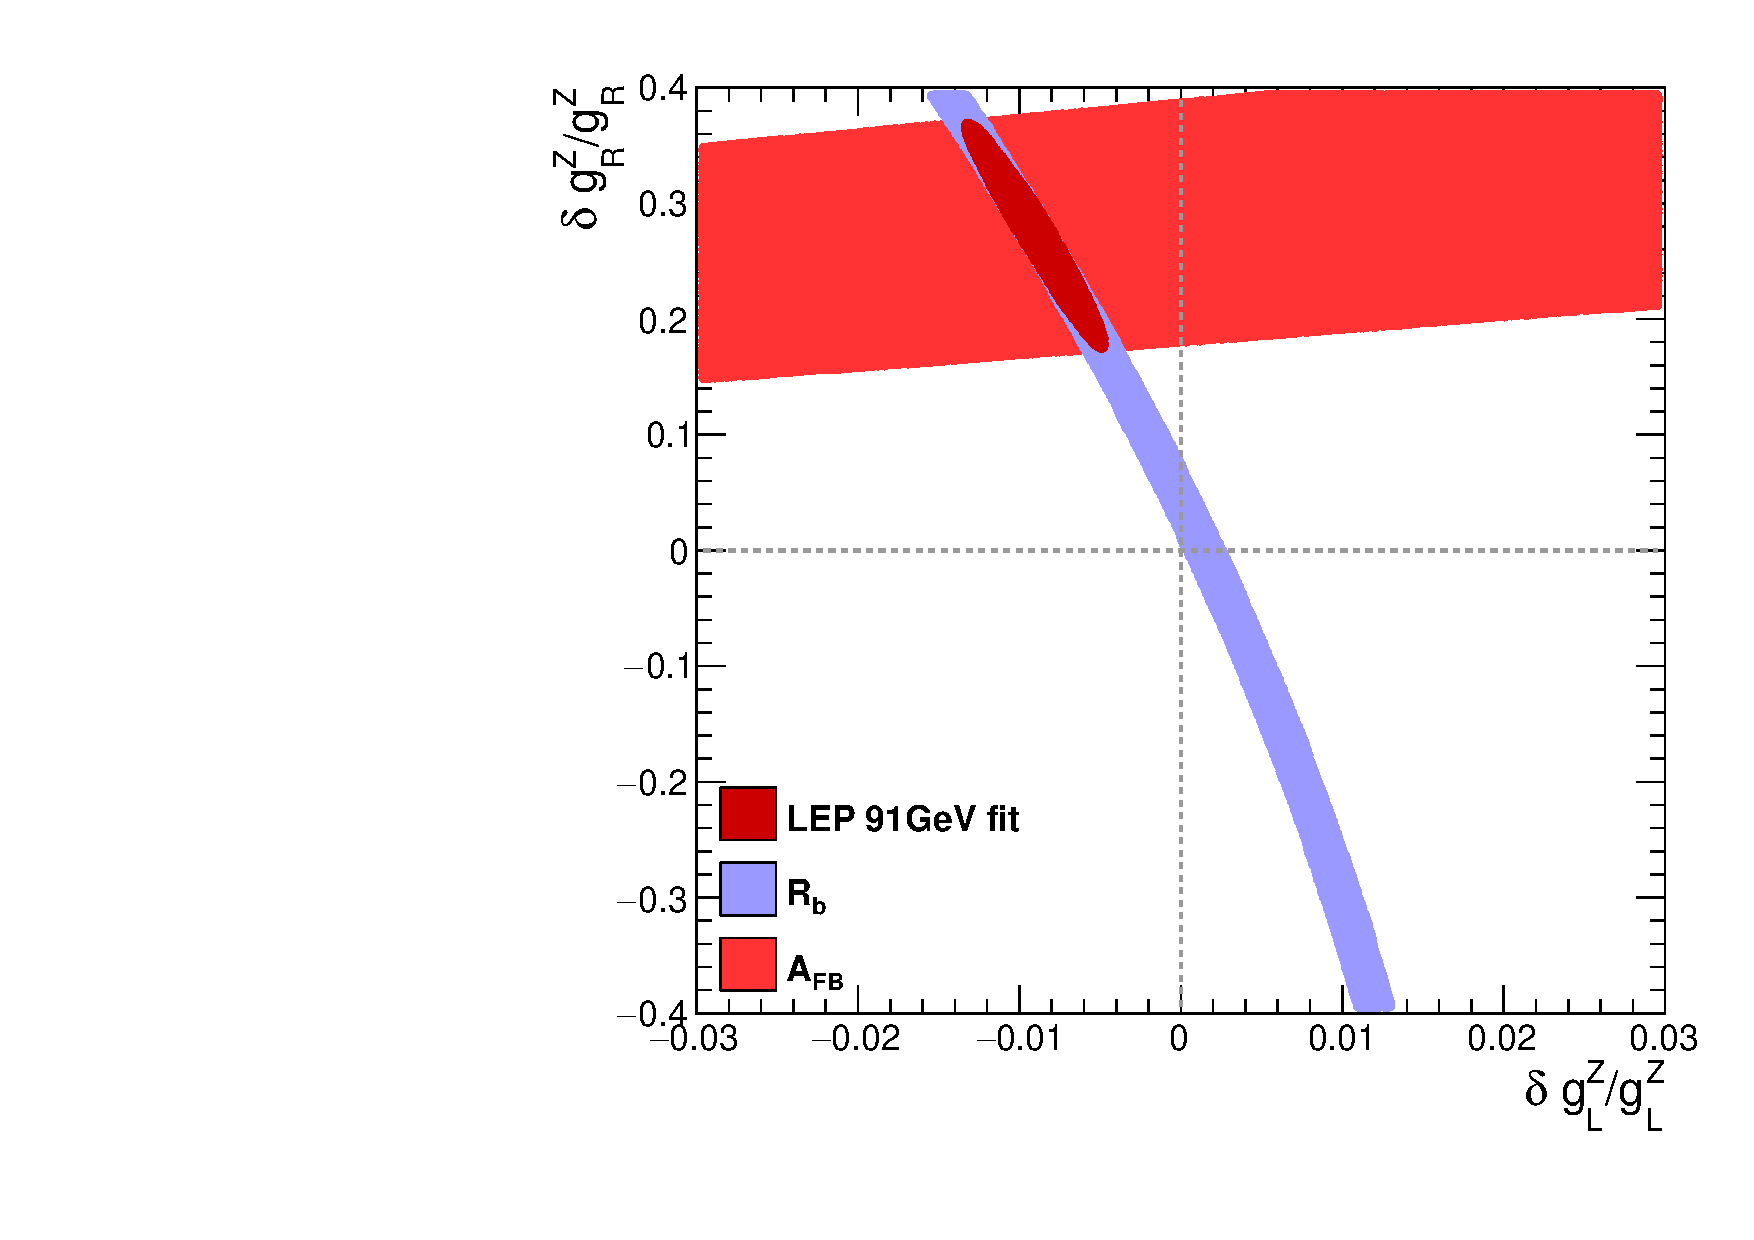
\includegraphics[width=0.4\linewidth]{../ILD/plots/lep-result-zoom.pdf}
	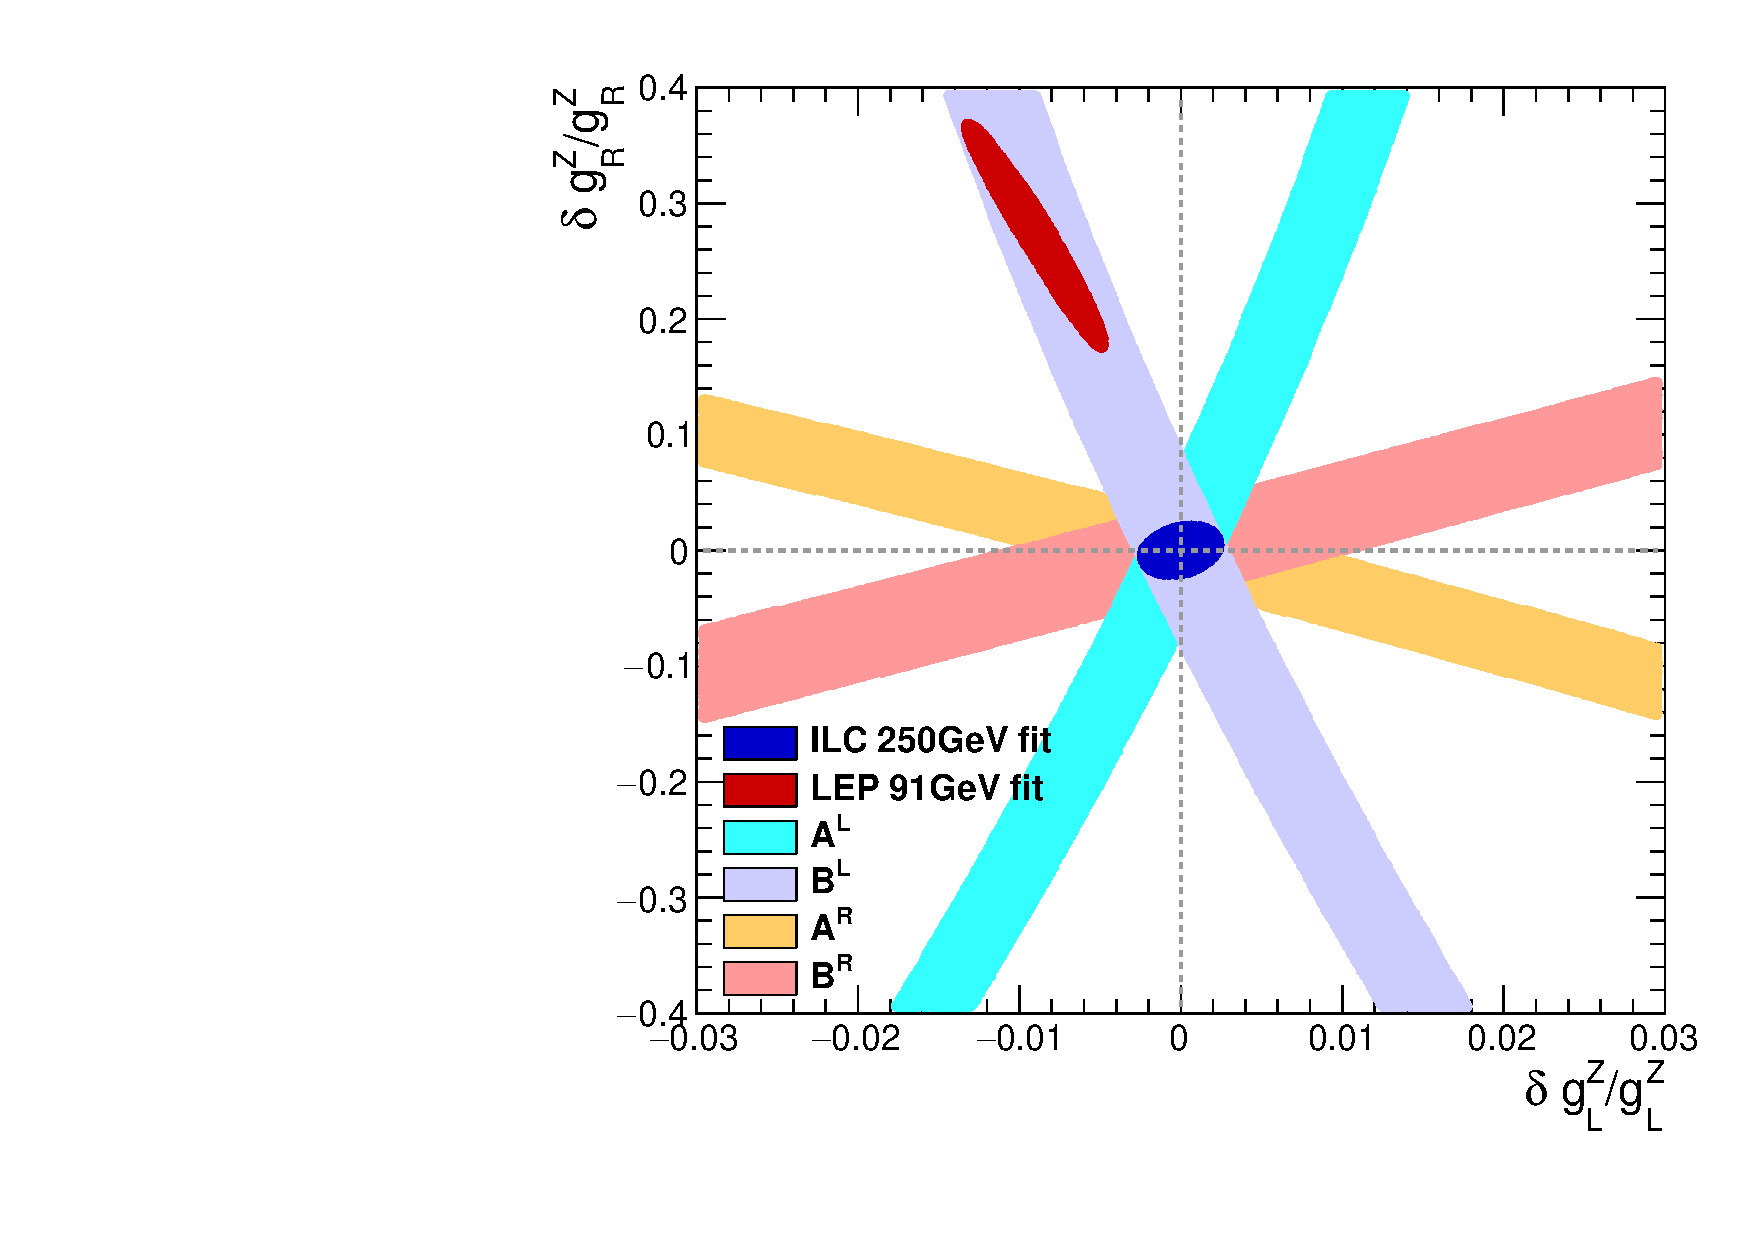
\includegraphics[width=0.4\linewidth]{../ILD/plots/ilc-result.pdf}
	\captionof{figure}{ Tree level $\pm 1\,\sigma$ allowed regions defined by the forward-backward asymmetry and total cross section measurements at LEP (left) and ILC via the differential cross section fit (right). Dashed guidelines show the \sm\ value. The allowed region expected at the ILC is centered at \sm\ values of couplings. }
		\label{fig:LEPILCResult_3}
\end{center}\vspace{1cm}

%----------------------------------------------------------------------------------------
%	CONCLUSIONS
%----------------------------------------------------------------------------------------

\color{SaddleBrown} % SaddleBrown color for the conclusions to make them stand out

\section*{Conclusions}

\begin{itemize}
\item Pellentesque eget orci eros. Fusce ultricies, tellus et pellentesque fringilla, ante massa luctus libero, quis tristique purus urna nec nibh. Phasellus fermentum rutrum elementum. Nam quis justo lectus.
\item Vestibulum sem ante, hendrerit a gravida ac, blandit quis magna.
\item Donec sem metus, facilisis at condimentum eget, vehicula ut massa. Morbi consequat, diam sed convallis tincidunt, arcu nunc.
\item Nunc at convallis urna. isus ante. Pellentesque condimentum dui. Etiam sagittis purus non tellus tempor volutpat. Donec et dui non massa tristique adipiscing.
\end{itemize}

\color{DarkSlateGray} % Set the color back to DarkSlateGray for the rest of the content

%----------------------------------------------------------------------------------------
%	FORTHCOMING RESEARCH
%----------------------------------------------------------------------------------------

\section*{Forthcoming Research}

Vivamus molestie, risus tempor vehicula mattis, libero arcu volutpat purus, sed blandit sem nibh eget turpis. Maecenas rutrum dui blandit lorem vulputate gravida. Praesent venenatis mi vel lorem tempor at varius diam sagittis. Nam eu leo id turpis interdum luctus a sed augue. Nam tellus.

 %----------------------------------------------------------------------------------------
%	REFERENCES
%----------------------------------------------------------------------------------------

%\nocite{*} % Print all references regardless of whether they were cited in the poster or not
\bibliographystyle{abbrv} % Plain referencing style
\bibliography{../mainbib} % Use the example bibliography file sample.bib

%----------------------------------------------------------------------------------------
%	ACKNOWLEDGEMENTS
%----------------------------------------------------------------------------------------

\section*{Acknowledgements}

Etiam fermentum, arcu ut gravida fringilla, dolor arcu laoreet justo, ut imperdiet urna arcu a arcu. Donec nec ante a dui tempus consectetur. Cras nisi turpis, dapibus sit amet mattis sed, laoreet.

%----------------------------------------------------------------------------------------

\end{multicols}
\end{document}